\section*{Aufgabe 2}

Es sollen das Intervallhalbierungs- und Newton-Verfahren mit einer Genauigkeitsschranke von jeweils \(x_\text{c} = \num{1e-9}\) implementiert werden. Getestet werden die beiden Verfahren an der Funktion
\begin{equation}
  f(x) = x^2-2, \label{eqn:f}
\end{equation}
deren analytisches Minimum bei \(x_\text{min} = 1\) liegt.
Für das Intervallhalbierungs-Verfahren werden die Startwerte \(a = \num{-0,5} \,, \: b = \num{-0,1}\) und \(c = 2\) verwendet.
In Abbildung \ref{fig:intervall} sind die Werte von \(a,b,c\) gegen die Anzahl der Iterationen aufgetragen.
\begin{figure}
  \centering
  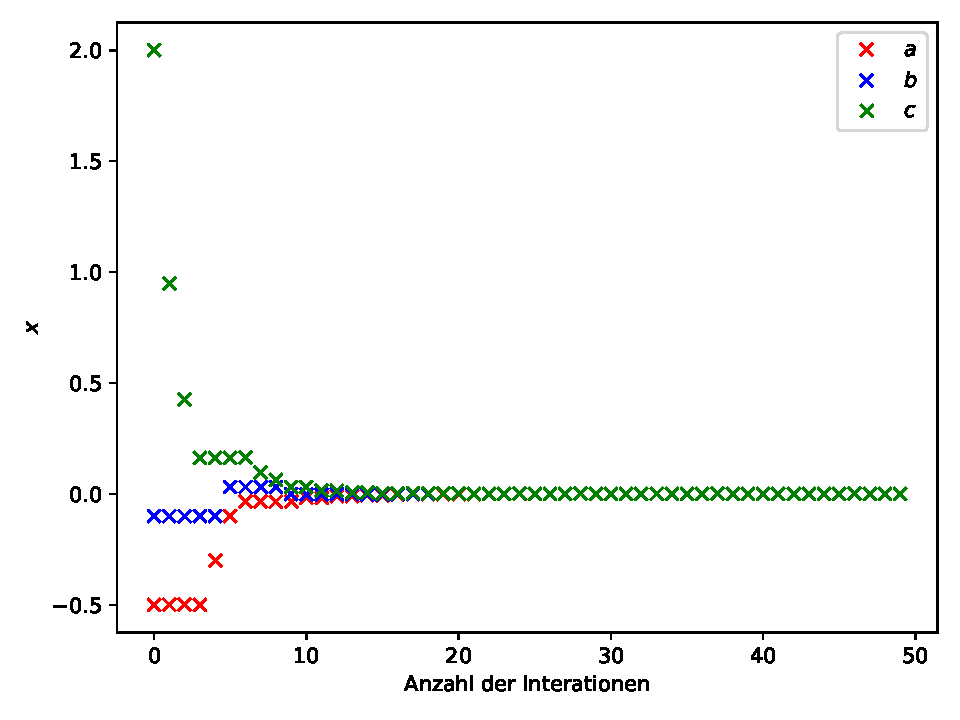
\includegraphics[width=0.45\textwidth]{A2/build/intervallhalbierung.pdf}
  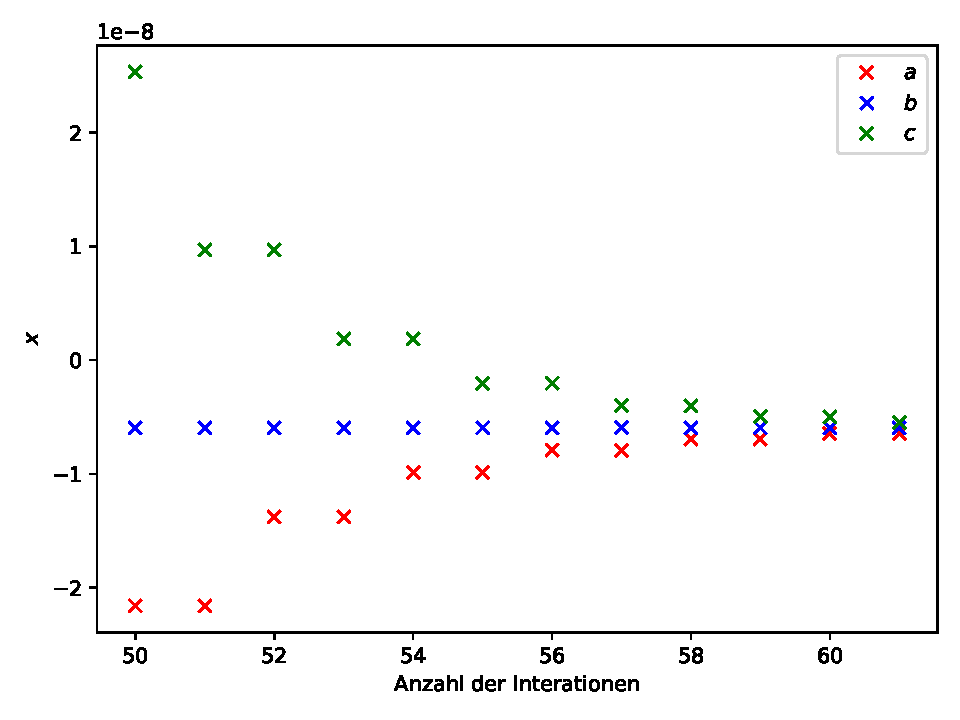
\includegraphics[width=0.45\textwidth]{A2/build/intervallhalbierung2.pdf}
  \caption{Intervallhalbierungs-Verfahren}
  \label{fig:intervall}
\end{figure}
Für das Newton-Verfahren wird der Startwert \(x_0 = 1\) verwendet. In Abbildung \ref{fig:newton} ist \(x_0\) gegen die Anzahl der Iterationen aufgetragen.
\begin{figure}
  \centering
  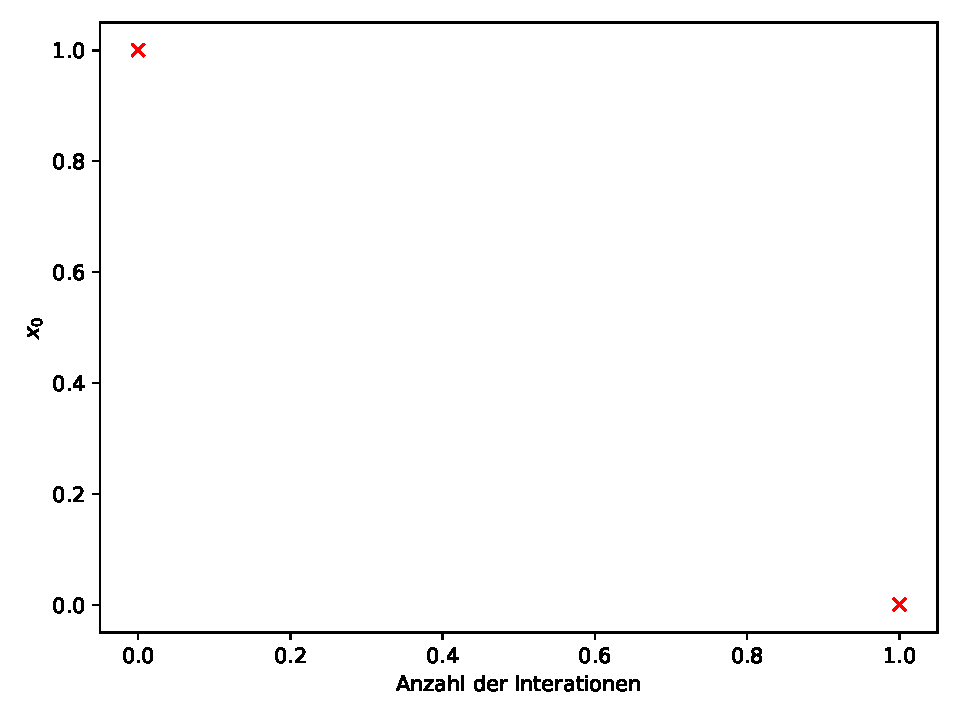
\includegraphics[width=0.7\textwidth]{A2/build/newton.pdf}
  \caption{Newton-Verfahren}
  \label{fig:newton}
\end{figure}
Das Newton-Verfahren erreicht schon nach der ersten Iteration die gewünschte Genauigkeit von \(\num{1e-9}\), während das Intervallhalbierungsverfahren dafür \(61\) Iterationen benötigt.
Mit einem Wert von \(x = \num{-8,22398e-11}\) liefert das Newton-Verfahren auch ein genaueres Ergebnis als das Intervallhalbierungs-Verfahren mit einem Intervall-Mittelwert von \(x = \num{-5,96047e-9}\).
Somit ist das Newton-Verfahren unter den vorgegebenen Anfangsbedingungen deutlich besser zur Minimierung der Funktion \eqref{eqn:f} geeignet.
